\documentclass{article}


\usepackage{authblk}
\usepackage[T1]{fontenc}
\usepackage{indentfirst}
\usepackage{graphicx}
\usepackage{amsmath}
\usepackage{caption}
\usepackage{hyperref}
\usepackage{float}
\usepackage{subcaption}


\begin{document}

\title{Photoluminescence}
\author[1]{Woojin Han}
\affil[1]{Seoul National University, Seoul 151-747, Korea}
\maketitle
\begin{abstract}
  In this experiment, photoluminescence(PL) of rhodamine 590 and ruby is measured.
  The apparatus establishment is improved, especially the role of the aperture is declared.
  The molecular orbital structure of rhodamine 590 and its Raman scattering is introduced.
  The fitting method is introduced and applied to the datum.
  The PL results of rhodamine 590 are plotted and each curve's nature has been explained.
  Analysis between PL peak statics of ruby and temperature is obtained and applied to experimental data.
  According to the peak intensity ratio specific energy gap is calculated.
\end{abstract}

\section{Introduction}
 Photoluminescence(PL) is one kind of luminescence on a sample.
 By the time taken in the emission of light, the luminescence is classified by fluorescence and photoluminescence.
 It is special because the wavelength of the light is changed by the event of absorption and emission.
 Therefore, detecting the PL results help us to find the structure basis in the scale of molecules or crystals.
 In this experiment, PL results of rhodamine 590 and ruby are measured and analyzed.

\subsection{Photoluminescence: General Theory}
 \label{intro:pl_general_theory}
 Photoluminescence is explained by two different parts, absorption and emission of light.
 Both events occur by the electronic transition through states, embedding the nature of the condensed matter.
 Therefore, the photoluminescence result leads us to measure the band diagram of the crystal.
 Not only the energy level of each band but also the lifetime or exact orbital can be measured by the peak statics, such as peak width or intensity ratio.
 \begin{figure}[ht]
    \centering
    \begin{subfigure}[b]{6cm}
        \centering
        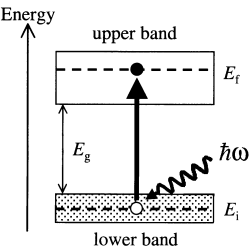
\includegraphics[width=4cm]{../results/intro_energy_absortion.png}
        \caption{}
    \end{subfigure}
    \hfill
    \begin{subfigure}[b]{6cm}
        \centering
        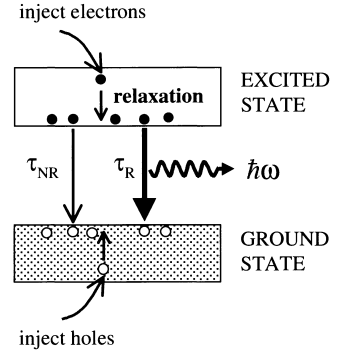
\includegraphics[width=4cm]{../results/intro_energy_emission.png}
        \caption{}
    \end{subfigure}
    \hfill
    \caption{Schematic diagram of (a)light absorption (b)light emission \cite{condensed_matter_optics}}
    \label{fig:pl_intro}
 \end{figure}

 \begin{figure}[ht]
    \centering
    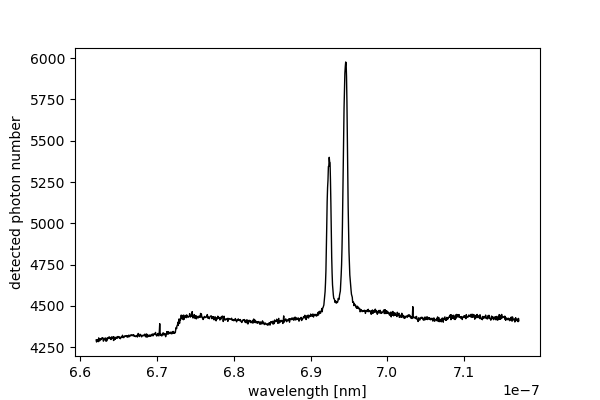
\includegraphics[width=8cm]{../results/Ruby(170.0)_raw_fig.png}
    \caption{photoluminescence results of Ruby in $170.0K$}
    \label{fig:pl_sample}
 \end{figure}
 Fig. \ref{fig:pl_intro}(a) shows the band diagram explanation of light absorption, creating a hole in the lower band transition to the upper band.
 Fig. \ref{fig:pl_intro}(b) is the schematic diagram of light emission, slowly relaxing and emitting light while energy drops between band gaps.
 Fig. \ref{fig:pl_sample} is one of the photoluminescence results in this experiment.
 The absorbed light was $532nm$, but we can find out the emitted light has a wavelength of around $690nm$.
 We can be sure the electronic transition is the key mechanism since the wavelength change can not be explained by scattering, especially for the peaked nature.
 Therefore, the peak position is specific to the crystal structure or the molecular shapes.
 But the peak width has two reasons, natural and optical broadening. (\cite{quantum_optics})
 Natural broadening is intrinsic to the transition, caused by the lifetime of the states.
 For lifetime $\tau$, the spectral function follows Lorentzian-like equation (\ref{equation:natural_broadening}), $\omega$ is the angular frequency of light, and $\Delta \omega$ is full width at half maximum(FWHM) value which is related with lifetime.
 \begin{equation}
   g(\omega) = \frac{\Delta \omega}{2 \pi} \frac{1}{(\omega-\omega_0)^2 + (\Delta \omega/2)^2},\, \Delta \omega = \frac{1}{\tau}
   \label{equation:natural_broadening}
 \end{equation}
 And by the spectral effects of spectroscopy itself, the Gaussian shape optical broadening is inevitable.
 Therefore, I assume that the detected photoluminescence spectroscopy data will follow the Voigt profile, which is a convolution result of the Lorentzian and Gaussian functions.


 \subsection{Ruby}
 \label{intro:ruby}
 In the theory of solid-state luminescence, simultaneous emission is allowed between special states.
 Otherwise, an electron can lose its energy in phonon which we call nonradiative transition.
 The phonon physics is explained by the Debye model, assuming that the highest frequency of phonon is restricted by the size of the lattice denoted as $\omega_D$.
 And phonon follows boson statics, which can easily induce the density of states.
 
 \begin{multline}
  H= \sum_{n=0}^3 \epsilon_n \psi_n^\dagger \psi_n + \sum_k (\hbar \nu k) (a_k a_k^\dagger + \frac{1}{2}) + S_0 (C_{12} \psi_1^\dagger + \sum_{n=1,2} C_{n3} \psi_n^\dagger \psi_3 + c.c.) \\
   + S_0^2 (\sum_{n=0}^2 d_n \psi_n^\dagger \psi_n + [d_{12}\psi_1^\dagger \psi_2 + c.c.])
  \label{equation:phenomenological_hamiltonian}
 \end{multline}

 In \cite{Ruby_temp_theoretical}, they declare the phenomenological Hamiltonian of impurity ruby as equation \ref{equation:phenomenological_hamiltonian}.
 As the two big peak is observed near $690nm$, we assume three excited-state levels $n=1,2,3$ have energy of $\epsilon_1, \epsilon_2, \epsilon_3$ and wave function of $\psi_1, \psi_2, \psi_3$ respectivly.
 The first term is about the electronic state's energy of impurity.
 The second term is phonon energy, which $k$ is bounded by Debye frequency.
 In ruby, the first and second excited states are $E_2$ levels and the photoluminescence peak appears by the spontaneous emission through $1\rightarrow0$ and $2\rightarrow0$.
 Empirically, $0=\epsilon_0 \ll \epsilon_1 < \epsilon_2 \ll \epsilon_3$, since the gren laser excites electron by $0\rightarrow3$ and by nonradiative $3\rightarrow1,2$ transition occurs.
 The leftover terms are suggested perturbation terms in \cite{Ruby_temp_theoretical}, assuming the doped $Cr^{3+}$ locates isotropic in the enlarged Debye model.
 In this experiment, the dopped ratio is small enough to fit in the assumption.
 \begin{multline}
  \epsilon_n (T) = \epsilon_n (0) + \alpha_n (\frac{T}{T_D})^4 \int_{0}^{T_D / T} dx \frac{x^3}{e^x -1} - \beta_{12} (-1)^n \frac{T_e}{T_D} (\frac{T}{T_D})^2 \\
  \times \int^{T_D/T}_{0} dx \frac{x^3}{e^x -1} \frac{P}{x^2 - (T_e/T_D)^2}
  \label{equation:peak_position}
 \end{multline}
 \begin{multline}
  \Gamma_n(T) = \Gamma_n(0) + \bar{\alpha_n} (\frac{T}{T_D})^7 \int^{T_D/T}_{0} dx \frac{x^6 e^x}{(e^x -1)^2}\\ + \pi \beta_{12} (\frac{T_e}{T_D})^3 [\delta_{n2}+\frac{1}{e^{T_e/T}-1}]
  \label{equation:peak_width}
 \end{multline}
 After calculating the lowest order of perturbation theory, we have the peak position in the function of temperature as equation \ref{equation:peak_position}.
 $T_D$ is Debye temperature, $\alpha_n , \beta_{12}$ is fitting coefficients, $T_e=(\epsilon_2 - \epsilon_1)/k_B$ is $42K$ in ruby.
 Equation \ref{equation:peak_width} shows the temperature dependence of each peak width, $\Gamma$ denotes the parameter of Lorentzian lineshape.
 $\bar{\alpha_n}$ is also a fitting variable, which has a direct expression to Hamiltonian coefficients.
 The first temperature perturbed term starting with $\alpha_n, \bar{\alpha_n}$ in both equations is a calculation of nonradiative effects.
 The second term starting with $\beta_{12}$ is the term of internal conversion between state $1,2$.
 In this case, the internal conversion can be disregarded, $\beta_{12}=0$.
 Specific fitting methods and results in this experiment are denoted below. (\ref{result:temperature_peak_statics})

 Those explanation doesn't imply the specific states, since we never come out with the crystal environments.
 Ruby is dopped crystal whose basic structure is built by $Al_2O_3$, hexagonal crystal structure, $Cr^{3+}$ located in an octahedral site.
 In this case, both crystal and ion energy states affect themselves to have broadband structures or energy splits.
 $Al_2 O_3$ doesn't have any fluorescence bandgaps, since we can never find photoluminescence peaks on other dopped ions.
 This means that the affected $Cr^{3+}$ energy structure is the key to this luminescence effect.
 Fig \ref{fig:ruby_band_structure}, adapted from \cite{Ruby_band_structure} shows the shift of ionic energy structure.
 The left side of the diagram is the original orbital energy of free $Cr^{3+}$.
 As the cubic field parameter $Dq/B$ increases, the energy level gets split and broadened.
 The diagram at $Dq/B=3$ represents the energy level of the $Cr^{3+}$ in ruby, which in this case doesn't split enough and is considered constant.
 So, $^4A_2 , ^2E, ^2T_1 , ^4T_2$ is the $\epsilon_0, \epsilon_1, \epsilon_2, \epsilon_3$ state respectivly as explained.
 As a conclusion, the dopped ruby absorbs green light to transmit electrons from $^4A_2 \rightarrow ^4T_2$ and nonradiative transit to $^4T_2 \rightarrow \,^2 T_1, \,^2E$ and give $R_1, R_2$ emitted light peak by $\,^2T_1, \,^2E \rightarrow \,^4A_2$. 

 \begin{figure}[ht]
  \centering
  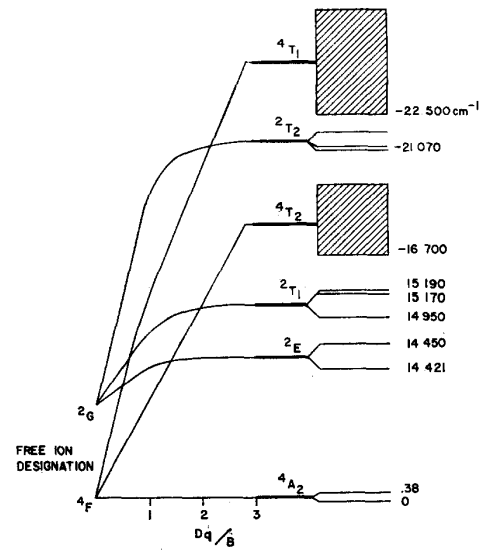
\includegraphics[width=6cm]{../results/ruby_band_diagram.png}
  \caption{Energy level diagram of $Cr^{3+}$ in ruby. adapted form \cite{Ruby_band_structure}}
  \label{fig:ruby_band_structure}
\end{figure}

By the vibrational state above $\,^2A$, the stokes sideband occurs.
In Fig. \ref{fig:pl_sample}, between $670 - 680 [nm]$ bump is that, have significant data with vibrational statics of the crystal.
But it is too wide so the spectroscopy results were cut to the right side of the band, therefore it is hard to declare exact measurements.
So in this report, I disregard the Stokes sideband in the analysis of peaks.


\subsection{Rhodamine 6G(R6G)}
 Rhodamine 6G (R6G) is one of the highly fluorescent triaryl methane dyes.
 Fig. \ref{fig:rhodamine_structure} shows the molecular structure of R6G.
 It has three benzene ring, which allows each atomic orbital forms a fluorescence conjugated system.
 In photochemistry, we assume the linear combination of each atomic orbital forms a molecular orbital.
 This means that the total Hamiltonian of the molecule is described by the function of linear coefficients.
 Therefore, the eigenstate of the Hamiltonian gives the energy diagram of a molecule.
 \begin{figure}[ht]
  \centering
  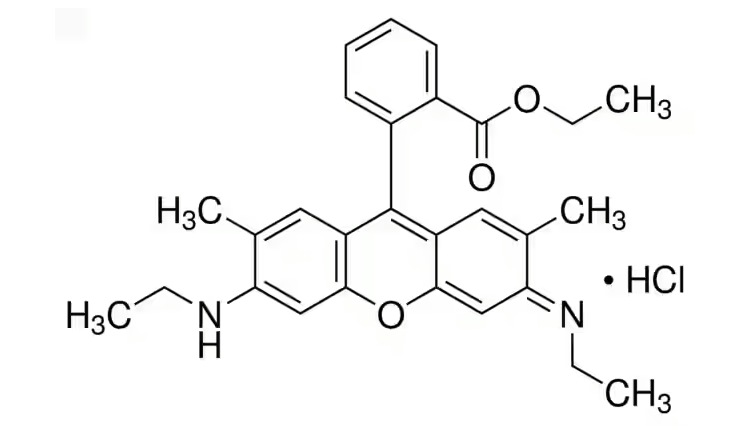
\includegraphics[width=6cm]{../results/Rhodamin_structure.png}
  \caption{Structural formula of R6G, adapted from \cite{rhodamine_sigma_aldrich}}
  \label{fig:rhodamine_structure}
 \end{figure}
 In this experiment, we dissolve R6G in ethylene glycol, which needs a different approach to ruby.
 Since the molecules do not fix their position, they can freely vibrate and rotate.
 Therefore, the PL results of R6G must consider a Raman shift.
 And also \cite{Rhodamine_dimer} reports that the concentration of the solution affects the peak position and FWHM.
 It declares a significant role of dimer formation by $\pi -\pi$ stacking interaction.
 But by Frank Condon's principle, the molecular position does not change while the electric transition occurs, the energy gap between monomer and dimer is disregarded.

 \begin{figure}[ht]
  \centering
  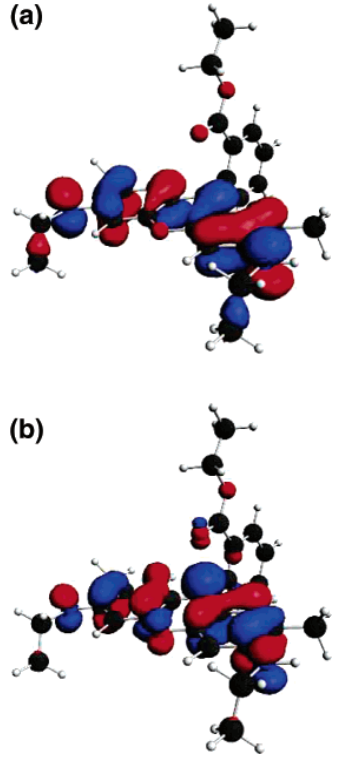
\includegraphics[width=4cm]{../results/Rhodamine_homo_lumo.png}
  \caption{The HOMO (a) and LUMO (b) of R6G adapted from \cite{rhodamine_HOMO_LUMO}}
  \label{fig:rhodamine_homo_lumo}
 \end{figure}

 In photochemistry, the nonradiative, and radiative transition can be explained once in the Jablonski diagram.
 Jablonski diagram has each vibrational mode in a multiplicity of states, denoted by $M = 2S+1$. $S$ is the total electric spin.
 For example, if the all-electron is in spin pair, $S=0, M=1$.
 It is a singlet state.
 By the value of $M=1,2,3,4, ... $ the state will name after singlet, doublet, triplet and so on.
 The state $\,^4S$ is the fourth excited state of the singlet.
 Fig. \ref{fig:rhodamine_homo_lumo} shows the highest occupied molecular orbital (HOMO) and lowest unoccupied molecular orbital (LUMO) of the R6G molecule.
 By definition, as the light irradiates the molecule electron excites over LUMO from HOMO.
 And, by nonradiative transition bringing down the excited electron to LUMO, the radiative transition between LUMO and HOMO makes luminescence.
 As Fig. \ref{fig:rhodamine_homo_lumo}, each Benzene ring switches its phase to have an energy gap near 560nm.
 The photoluminescence transition is $\,^1S \rightarrow \,^0S$, spin unchanged.

\section{Methods}
 The photoluminescence module has been set up in the intermediate physics experiment laboratory, at Seoul National University.
 The laser is from Shanghai Dream Lasers Technology Co., Model is SDL-532-030T (\cite{laser_spec}), maximum power of $30mW$ and a low noise feature.
 Compressor is from CSIC Pride (Nanjing) Cryogenic Technology Co., Model is KDC 2000F (\cite{compressor_spec})
 The CCD camera is from Andor, Model is DV401A-BVF (\cite{ccd_spec}), which secures 99\% linearity of photon detection.
 Spectrograph is from Dongwoo Optron Co., Model is MonoRa500I (\cite{spectrograph_spec}).
 Spectrograph has four slits, two of which were closed.
 Its slit can be modified by the micrometer attached to each entrance.
 The modification is limited to opening up an aperture, not the specific details of the spectrograph.
 Fig. \ref{fig:apparatus_sketch}(a) shows the brief structure of the spectrograph.
 In this experiment, I close the left aperture by setting the dial to $-0.1mm$.
 The black arrow is the path of a laser in Fig. \ref{fig:apparatus_sketch}(b).
 The laser emitted from below split by the dichroic filter encounters to sample.
 Sample scatters light in every direction, but the diagram only shows the useful light ray which goes into the Notch filter.
 Each dichroic filter and Notch filter selects the appropriate wavelength for each sample.
 I measure R6G soluted in ethylene glycol and ruby at room temperature, standard pressure.

 \begin{figure}[ht]
  \centering
  \begin{subfigure}[b]{6cm}
      \centering
      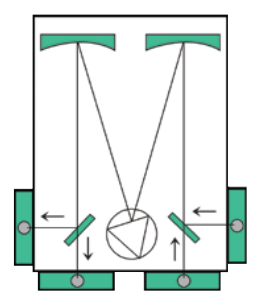
\includegraphics[width=3cm]{../results/spectrograph_sketch.png}
      \caption{}
  \end{subfigure}
  \hfill
  \begin{subfigure}[b]{6cm}
      \centering
      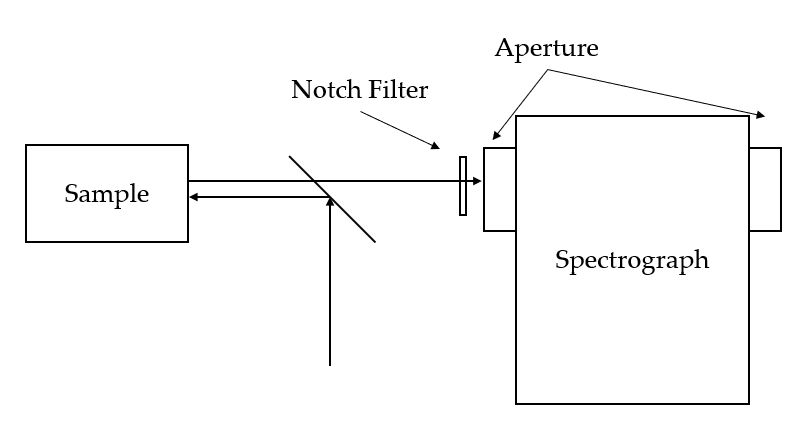
\includegraphics[width=6cm]{../results/total_module_sketch.png}
      \caption{}
  \end{subfigure}
  \hfill
  \caption{Schematic diagram of (a) spectrograph, adapted form  \cite{spectrograph_spec} (b)total photoluminescence module}
  \label{fig:apparatus_sketch}
\end{figure}


\subsection{Ruby: PL by temperature}
 I fix the alignment and set the sample pressure under 10mTorr using the rotary pump.
 Then using a compressor, lower the sample temperature from $270K$ to $10K$.
 If the grating speed is too fast, turn on the heater attached to the sample to mediate the speed.
 I detect photons from the CCD camera for every $5K$ and read the middle temperature of detection while proceeding.
 In this experiment, about $0.2K$ has cooled so the photoluminescence by temperature detection is vouched by the accuracy of $0.1K$.


\section{Results and Discussion}\

All of the results are uploaded at \cite{github_results}.
In this report, some sample plots are attached, which do not influence the generality of logical flows.
The file name and detailed contents are tables in Fig. \ref{fig:file_appendix}

\begin{figure}[H]
  \centering
  \begin{tabular}{|c|c|}
      file name  & details \\
      \hline
      \verb|Ruby sx-y_raw_fig.png| & Ruby PL plot of slit width $x$ in repeated index $y$\\
      \verb|R6G(x)_raw_fig.png| & R6G PL plot of repeated index $x$, raw figure\\
      \verb|R6G(x)_gaussian_fitted_fig.png| & R6G PL plot of repeated index $x$ gaussian fitted figure\\
      \verb|Ruby(T)_raw_fig.png| & Ruby PL plot in temperature $T$ , raw  figure\\
      \verb|Ruby(T)_voigt_fitted_fig.png| & Ruby PL plot in temperature $T$, Voigt fitted figure\\
      \verb|R6G_total_fig.png| & United plot of R6G sample\\
      \verb|Ruby_temperature_peak_fig.png| & United plot of Ruby sample, peak position statics\\
      \verb|Ruby_temperature_width_fig.png| & United plot of Ruby sample, peak width statics\\

  \end{tabular}
  \caption{file appendix of \cite{github_results}}
  \label{fig:file_appendix}
\end{figure}

\subsection{Aperture setting}
\label{result:aperture_effect}
 I repeatedly measure the ruby sample in the same temperature, pressure and alignment condition, only changing the aperture slit width.
 Fig. \ref{fig:s5_s30_difference} shows two extreme cases of $0.05 mm$ and $0.30 mm$ opened results.
 As the aperture is closed, fewer photons are detected, and the peaks do not dominate the results.
 But, the widely opened aperture makes the resolution worse.
 In this trade-off, we choose to take the slit width of $0.25 mm$, since the Stokes sideband is significantly observable from that width.
 This leads us to expect the minor band can be visible through the noise either.
 

 \begin{figure}[ht]
  \centering
  \begin{subfigure}[b]{6cm}
      \centering
      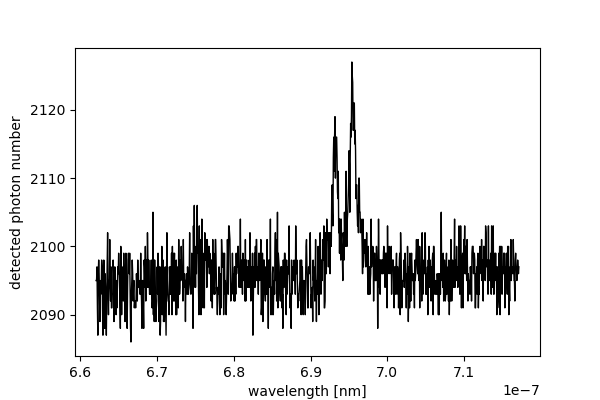
\includegraphics[width=6cm]{../results/Ruby s5-1_raw_fig.png}
      \caption{}
  \end{subfigure}
  \hfill
  \begin{subfigure}[b]{6cm}
      \centering
      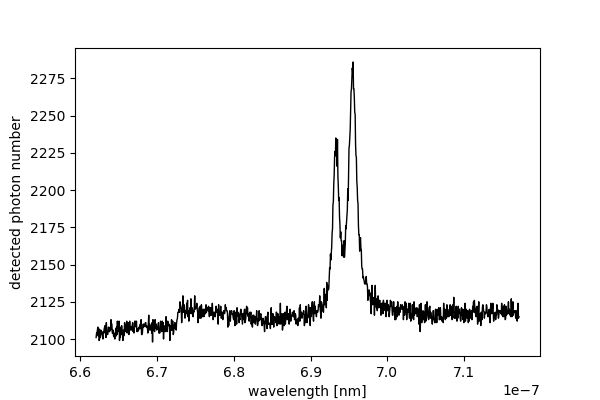
\includegraphics[width=6cm]{../results/Ruby s30-1_raw_fig.png}
      \caption{}
  \end{subfigure}
  \hfill
  \caption{PL result of ruby in (a)0.05mm (b)0.30mm opened aperture}
  \label{fig:s5_s30_difference}
\end{figure}
 
\subsection{Rhodamin 6G}
 Fig. \ref{fig: R6G results}(b) shows the counts - energy [$eV$] plot and its Gaussian trend line.
 Peak statics of five repeated detection is provided in Fig. \ref{fig: R6G optimize results}.
 $N(E) = A \frac{1} {\sigma \sqrt{2\pi}} e^{-\frac{1}{2} \frac{(E-E_0)^2}{\sigma^2}}$ values are obtained.
 The amplitude $A$ and background light coefficient $C$ do not inform critical phenomena for R6G, the peak position and FWHM only matter.
 The band gap betwen LUMO and HOMO is $2.211 \pm 0.001$ [$eV$] and its lifetime is $(7.15 \pm 0.02) \times 10^{-15} $[$s$].
 \begin{figure}[ht]
  \centering
  \begin{subfigure}[b]{6cm}
      \centering
      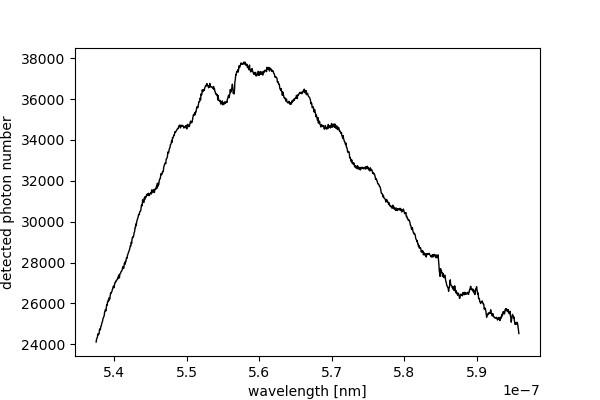
\includegraphics[width=6cm]{../results/R6G(1)_raw_fig.png}
      \caption{}
  \end{subfigure}
  \hfill
  \begin{subfigure}[b]{6cm}
      \centering
      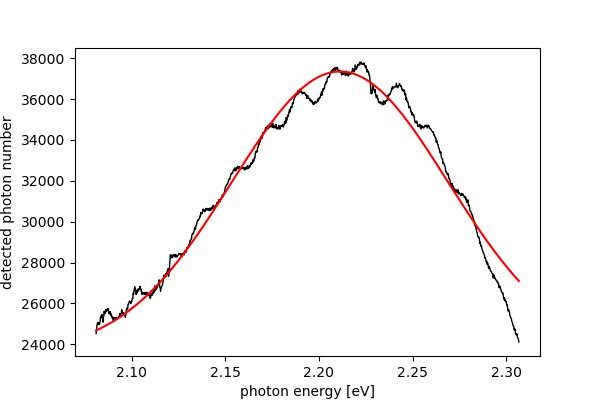
\includegraphics[width=6cm]{../results/R6G(1)_gaussian_fitted_fig.png}
      \caption{}
  \end{subfigure}
  \hfill
  \caption{PL result of R6G (a)counts - wavelength[$nm$] (b)counts - photon energy[$eV$]}
  \label{fig: R6G results}
\end{figure}

\begin{figure}[H]
  \centering
  \begin{tabular}{|c| c| c|c|c|}
      index  & $E_0 $[$eV$]  & $\sigma$ [$eV$] & $A$ & $C$\\
      \hline
      1 & $2.211$ & $5.78\times 10^{-2}$ & $1.99 \times 10^3$ & $2.36 \times 10^4$\\
      2 & $2.211$ & $5.77\times 10^{-2}$ & $2.10 \times 10^3$ & $2.47 \times 10^4$\\
      3 & $2.211$ & $5.77\times 10^{-2}$ & $1.92 \times 10^3$ & $2.30 \times 10^4$\\
      4 & $2.211$ & $5.77\times 10^{-2}$ & $2.03 \times 10^3$ & $2.41 \times 10^4$\\
      5 & $2.211$ & $5.76\times 10^{-2}$ & $2.06 \times 10^3$ & $2.45 \times 10^4$\\
      
  \end{tabular}
  \caption{Statics of Gaussian fitting of Fig. \ref{fig: R6G results} in different trials}
  \label{fig: R6G optimize results}
\end{figure}

The bumps on the peak are not random but keep appearing in repeated measurements.
Fig. \ref{fig: R6G total fig}(a) is the total plot of every datum in one plot.
We can check that the same sidebands are at the same position in different experiments.
I have rotated the vials and moved the position of the solution during the experiment, it does not relate to outer results.
Therefore, I assume those sidebands are related to Raman scattering.
The Raman shift of R6G is calculated in \cite{rhodamine_HOMO_LUMO}.
As the molecule in solution moves freely in ethylene glycol, the cross-section of the band gap might Raman shifted.
There are around 10-12 big peaks on the Raman shift as shown in Fig. \ref{fig: R6G total fig}(b), which are the same numbers as the experimental data.
Also, the dimer effect is reported from \cite{Rhodamine_dimer}, but in this experiment, the solution is diluted enough to ignore the dimer effects.

 \begin{figure}[ht]
  \centering
  \begin{subfigure}[b]{6cm}
      \centering
      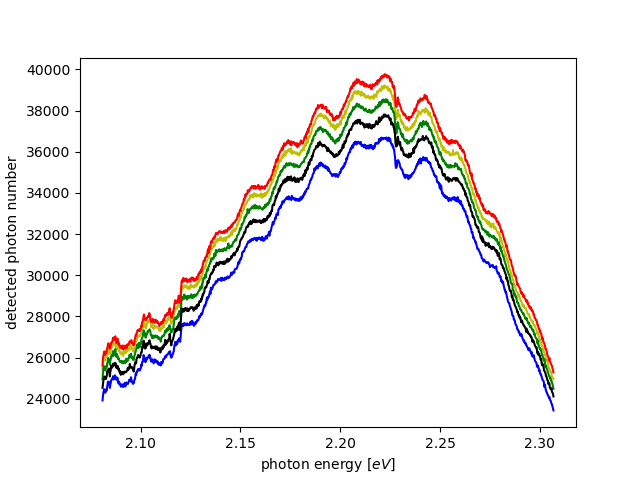
\includegraphics[width=6cm]{../results/R6G_total_fig.png}
      \caption{}
  \end{subfigure}
  \hfill
  \begin{subfigure}[b]{6cm}
      \centering
      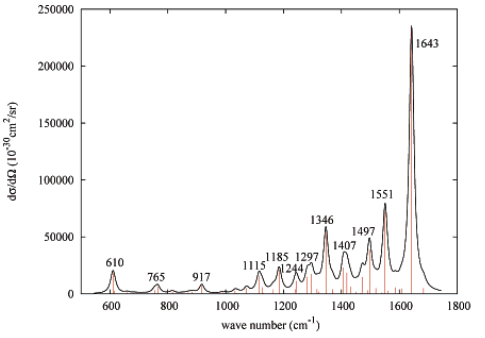
\includegraphics[width=6cm]{../results/Raman_shift.png}
      \caption{}
  \end{subfigure}
  \hfill
  \caption{(a)United plot of R6G PL data each color are the repeated measurements. (b)Raman shift calculation adapted from \cite{rhodamine_HOMO_LUMO}}
  \label{fig: R6G total fig}
\end{figure}

\subsection{Ruby PL result by temperature}
\label{result:temperature_peak_statics}  
 PL data of ruby for 51 different temperatures are measured.
 Fig. \ref{fig: Ruby_fitted_data} shows four representative PL plots of temperature 260.0, 190.0, 100.0, 6.00 K, and 6.0 [$mTorr$].
 As the sample temperature goes down, the peaks get sharper and can find the subtle peak position shift.
 Unlike the left peak, the R1 peak, the right peak, and the R2 peak get smaller so that at 6.0K, the R2 peak is hard to find in noises.
 The fitting eqauation $N(E)=A_1 V(E-E_1;\sigma,\gamma_1) + A_2 V(E-E_2;\sigma,\gamma_2)+C$, where $V(x;\sigma,\gamma)$ is Voigt profile.
 Fitting parameters are $E_1$ R1 peak position, $\gamma_1$ R1 peak Lorentzian FWHM and $A_1$ is the total photon number of the R1 peak.
 The same definition belongs to the R2 peak.
 And $\sigma$ is the Gaussian variance coefficient, which must be the same for both peaks.
 At extremely low temperatures, the R2 peak is gone so those values are fitted by one Voigt profile and R2 peak statics are set as NaN values.
 As this fitting assumes that the spectrograph errors are calculated in the parameter $\sigma$, the $\sigma $[$eV$] to sample temperature does not have any relation.
 Unfortunately the optical broadening, $\sigma$ is not equal to each temperature, but has some tendency with temperatures.
 I think that Voigt function fitting is very fragile to have a lot of optimized parameters so that $\sigma$ has a dependency on sample temperature.
 Although it is totally fine since the Voigt profile is normalized itself so that the amplitude directly means the peak area.

 \begin{figure}[ht]
  \centering
  \begin{subfigure}[b]{6cm}
      \centering
      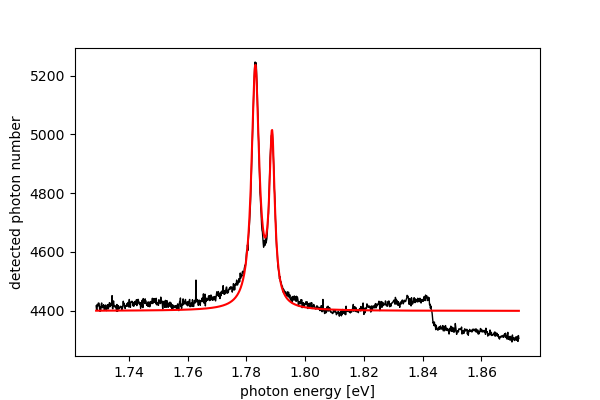
\includegraphics[width=6cm]{../results/Ruby(260.0)_voigt_fitted_fig.png}
      \caption{}
  \end{subfigure}
  \hfill
  \begin{subfigure}[b]{6cm}
      \centering
      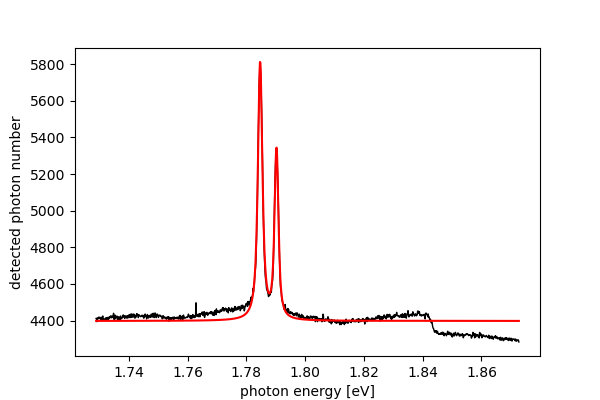
\includegraphics[width=6cm]{../results/Ruby(190.0)_voigt_fitted_fig.png}
      \caption{}
  \end{subfigure}
  \hfill
  \begin{subfigure}[b]{6cm}
    \centering
    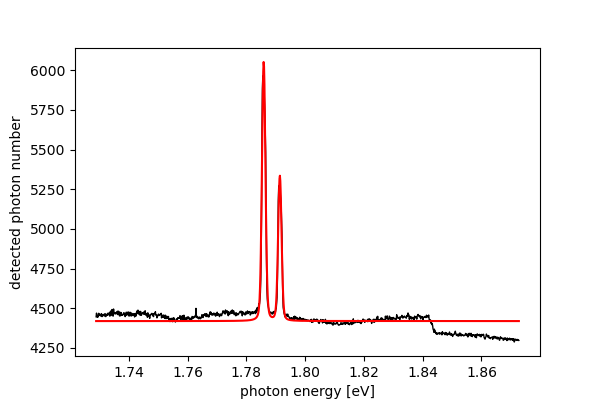
\includegraphics[width=6cm]{../results/Ruby(100.0)_voigt_fitted_fig.png}
    \caption{}
\end{subfigure}
\hfill
\begin{subfigure}[b]{6cm}
  \centering
  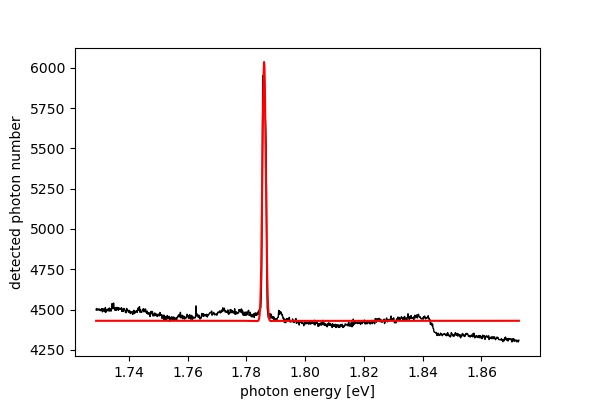
\includegraphics[width=6cm]{../results/Ruby(9.2)_voigt_fitted_fig.png}
  \caption{}
\end{subfigure}
\hfill
  \caption{Ruby PL data of pressure 6.0mTorr, and temperature (a)260.0K (b)190.0K (c)100.0K (d) 6.00K, in count - energy [$eV$] scale and its Voigt fitting results (red)}
  \label{fig: Ruby_fitted_data}
\end{figure}

Fig. \ref{fig: Ruby_temperature_results} shows the temperature dependence of each peak, and error bars are attached to each data point.
The error is propagated from the CCD camera resolution, every energy detection should have a measurement error of $0.0001$ [$eV$].
The error from the fitting calculation has an order of $10^{-10}$ [$eV$], which is very small.
By using equation \ref{equation:peak_position} and \ref{equation:peak_width}, $\epsilon_n(0)$ and $\alpha_n$, $\Gamma_n(0)$ and $\bar{\alpha_n}$ are fitted.
As the assumption from \cite{Ruby_temp_theoretical}, internal conversion coefficients $\beta_{12}$ has been disregarded as 0.
And also, Debye temperature $T_D$ can be calculated from the specific heat of $\alpha-Al_2 O_3 $ which is $760 K$.
Therefore, the peak positions at 0$K$ are $1.7861 \pm 0.0001$, $1.7916 \pm 0.0001$[$eV$].


Peak width is not clear enough, since Voigt profile is duplicated by various values of $\gamma$ and $\sigma$.
And, the Stokes sideband makes fitting goes to local optimal parameters, not the exact value of it.
So, I suggest using modified width defined by $\gamma^2 + \sigma^2$.
With the assertion that those value doesn't change a lot since $\sigma \ll \gamma$ holds.
Therefore, the peak widths at 0$K$ are $(5.6 \pm 0.5)\times 10^-4$, $(5.5 \pm 0.5)\times 10^-4$ [$eV$].
The lifetime of $^T_1 \rightarrow ^4A_2$ is $7.6 \times 10^{-11}$ s, $ ^2E \rightarrow ^4A_2$ is $7.7 \times 10^{-11}$s each.
That lifetime has an order of $10^-{11}$ s, which is appropriate for luminescence transition.

$\alpha_1 = -0.0928 \pm 0.0001$, $\alpha_2 = -0.0875 \pm 0.0001$ [$eV$], $\bar{\alpha_1} = 0.3275 \pm 0.0001$, $\bar{\alpha_2} = 0.1901 \pm 0.0001$ [$eV$] values are also fitted.
Those values have information of $Cr^{3+}$ impurity values by calculation of \cite{fitting_coef_impurity}.
Unfortunately, the experimental results by $\alpha_n$ to impurity are not available since modifying the impurity of ruby crystal is too hard.
But in \cite{doping_ratio}, the clever method has been suggested.
They form a ceramic cube of $Al_2 O_3$ in different mole fractions of $Cr^{3+}$ and measure PL.
But it is not a clean crystal and amorphous, and does not have a clean peak like the ruby sample.
Therefore in this report, I will leave the mole fraction analysis behind.

\begin{figure}[ht]
  \centering
  \begin{subfigure}[b]{6cm}
      \centering
      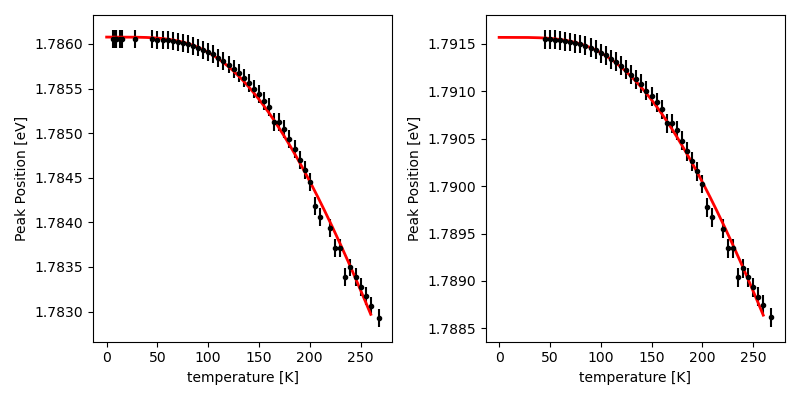
\includegraphics[width=6cm]{../results/Ruby_temperature_peak_fig.png}
      \caption{}
  \end{subfigure}
  \hfill
  \begin{subfigure}[b]{6cm}
      \centering
      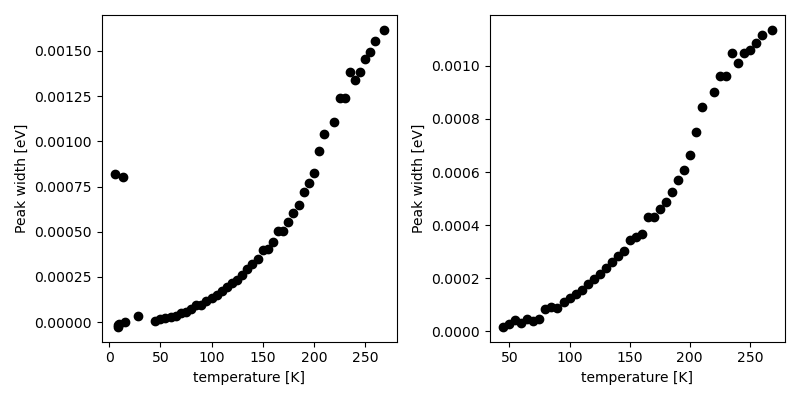
\includegraphics[width=6cm]{../results/Ruby_temperature_width_fig.png}
      \caption{}
  \end{subfigure}

  \caption{(a) peak position [$eV$] (b) peak width [$eV$] to sample temperature [K] plot. R1(left), R2(right), red lines are the appropriate fitted functions.}
  \label{fig: Ruby_temperature_results}
\end{figure}

\subsection{Peak Height Ratio}
\label{results: peak_height}

To analysis on the peak's area, it seems like the normalized property of the Voigt profile might help, but the redundancy of the Voigt profile ruins the overlapped region.
In each, the redundant parameter of the profile calculates the overlapped region differently.
So, I can not declare the selection of one optical broadening value separately from other values, Therefore I used the peak height data to explain physics itself.
It perfectly removes the duplicate effect of the optical broadening.
Fig. \ref{fig: ruby_temperature_height_ratio}(a) shows the raw plot of the experiment.
To calculate energy gap data from the results, \ref{fig: ruby_temperature_height_ratio}(b) plots the $log I_2/I_1$ - $1/T [1/K]$, where $I_1 , I_2$ is the height of $R_1, R_2$ respectivly.
$I_2/ I_1$ follows $A e^{-\frac{\Delta E}{kT}}$ theoretically, $log(I_2/I_1) = -\frac{\Delta E}{k} \frac{1}{T} + log(A)$.
Linear regression results is followed. $-\frac{\Delta E}{k} = 34.2 \pm 0.7 [K]$ and $log(A) = -0.263 \pm 0.006$ in R-value $0.992$.
Therefore the energy gap difference of the excited states is $\Delta E =(2.94 \pm 0.06) \times 10^{-3} [eV]$ by peak height data.

\begin{figure}[ht]
  \centering
  \begin{subfigure}[b]{6cm}
    \centering
    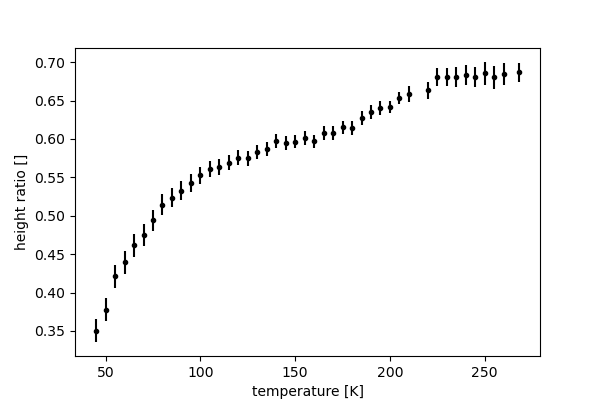
\includegraphics[width=6cm]{../results/Ruby_temperature_height_ratio_fig.png}
    \caption{}
  \end{subfigure}
  \hfill
  \begin{subfigure}[b]{6cm}
      \centering
      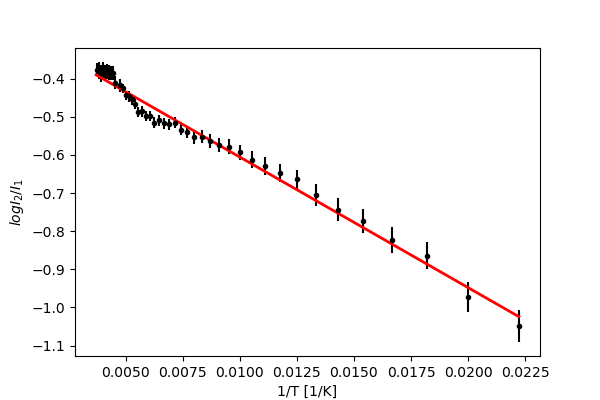
\includegraphics[width=6cm]{../results/Ruby_temperature_height_ratio_loglog_fig.png}
      \caption{}
  \end{subfigure}
  \caption{(a) $I_1/I_2$ - temperature [$K$], and (b)its reciprocal plot, the red line is a linear regression of $R^2 = 0.9924$}
  \label{fig: ruby_temperature_height_ratio}
 \end{figure}

\section{Summary}
The PL results of R6G and ruby are measured.
The optimal slit setting is measured and the optimal apparatus setup is detailed.
HOMO and LUMO of R6G molecule are cited, and the specific spin nature is explained.
In the PL plot of R6G, the repeated curve is reported and explained by Raman scattering.
The PL results of ruby are fitted by the Voigt profile, and its redundant limitation is observed.
The specific $Cr^{3+}$ energy diagram with field density $Dq/B$ is adapted.
Therefore, the specific transition of each peak, $R_1, R_2$ is obtained.
By using a three-level model, temperature dependence of peak statics is applied and checked with experimental data.

 
 
\bibliography{photoluminescence_ref}
\bibliographystyle{plain}
\end{document}